\documentclass[10 pt]{article}
\usepackage{multicol}
\usepackage[ portrait, margin = 0.7 in]{geometry}
\usepackage{graphicx}
\usepackage{float}
\usepackage[justification=centering]{caption}
\usepackage{amsmath}
\usepackage{subfig}
\usepackage{gensymb}
\usepackage{amssymb}
\usepackage{url}
\graphicspath{ {image2/}} 
\numberwithin{equation}{section}

\begin{document}


\title{\LARGE \bf Computational Physics \\ Exercise 2 : Partial Differential Equations }
\author{MERCIER Wilfried  -  University of Bristol}

\maketitle


\begin{abstract}

The aim of this work is to study partial differential equations using finite difference algorithms. We start by looking at Laplace's equation in 2D and we solve it with a boundary condition for which there exists an analytic solution using relaxation method. We compare the result to the analytic solutions and we investigate its performances. We then use it to determine the potential and the electric field within and around a plate capacitor. We compare the solution to the analytic one and see how it behaves when the capacitor can be approximated by an infinite sheet in both directions.
Finally we determine the heat distribution of an iron poker in function of time in two different cases by solving the heat equation using a fully implicit method.

\end{abstract}

\begin{multicols}{2}

\section{Laplace's equation}
\subsection{Discretized Laplace's equation}

We are interested in solving numerically Laplace's equation in two dimensions

\begin{equation}
\nabla ^2 V = \frac{\partial ^2 V}{\partial x^2} + \frac{\partial ^2 V}{\partial y^2} = 0
\end{equation}

Where V is the potential. If we want to find a solution on a domain $D : [0,x_N] \times [0,y_N]$\footnote{Others domains can be obtained by making the change of variables $x \rightarrow x + x_0$ and $y \rightarrow y + y_0$ and by stretching $x_N$ and $y_N$ by the appropriate factors} we need to know the boundary conditions of V on $\partial D$. This can be done by either putting the boundaries to a certain value (Dirichlet's conditions) or define the normal derivative at the boundaries (Neumann's conditions) or a mix of both. For simplicity we will only consider the following Dirichlet's conditions

\begin{equation}
\begin{split}
&V(0,y) = 0,\ \ V(x_N, y) = 0\\
&V(x, 0) = 0,\ \ V(0, y_N) = \sinh \frac{\pi x}{x_{N}}
\end{split}
\end{equation}

We will have to find discrete expressions for the second derivatives in Laplace's equation in order to write an algorithm. This can be done by looking at the Taylor expansions of V around $x\pm h$ and $y\pm h$ \cite{ComputationalTechnics}. Let us first look at the expansions around $x+h$ and $y+h$

\begin{equation}
\begin{split}
& V(x+h,y) = V(x,y)+h \frac{\partial V}{\partial x}  +\frac{h^2}{2}   \frac{\partial^2 V}{\partial x} +o(h^2)\\
& V(x,y+h) = V(x,y)+ h \frac{\partial V}{\partial y}  + \frac{h^2}{2}  \frac{\partial^2 V}{\partial y} +o(h^2)
\end{split}
\end{equation}

One can see that the expansions around $x-h$ and $y-h$ will leave the zeroth and second orders unchanged but will swap the sign of the first order. Hence by adding the two expansions we get two new equations

\begin{equation}
\begin{split}
&V(x+h,y) + V(x-h,y) = 2 V(x,y) + \hbar^2 \frac{\partial^2 V}{\partial^2 x}\\
&V(x,y+h) + V(x,y-h) = 2V(x,y) + \hbar^2 \frac{\partial^2 V}{\partial^2 y}
\end{split}
\end{equation}

In order to find a numerical solution, we need to discretize our domain D. We therefore define a grid of points $(i,j)$ such that $V(x,y) = V_{ij}$. We denote by h the step in both x and y directions between two adjacent points $h = V_{i+1, j} - V_{ij} = V_{i, j+1} - V_{ij}$. \\
Hence we can rewrite our Laplacian using Equation 1.4

\begin{equation}
\nabla^2 V \approx \frac{V_{i+1,j} + V_{i-1,j} + V_{i,j+1} + V{i,j-1} - 4V_{ij}}{h^2}
\end{equation}

And from Laplace's equation we get an expression to calculate each $V_{ij}$ on the grid

\begin{equation}
V_{ij} \approx \frac{V_{i+1,j} + V_{i-1,j} + V_{i,j+1} + V_{i,j-1}}{4}
\end{equation}

This corresponds to the average of the four points around $(i,j)$ and therefore it cannot be applied to the boundaries of the domain. This is an approximated solution and it will therefore depends upon the choice of h. Hence we should expect that the denser the grid the more accurate the approximation.

\end{multicols}

\begin{figure}[H]
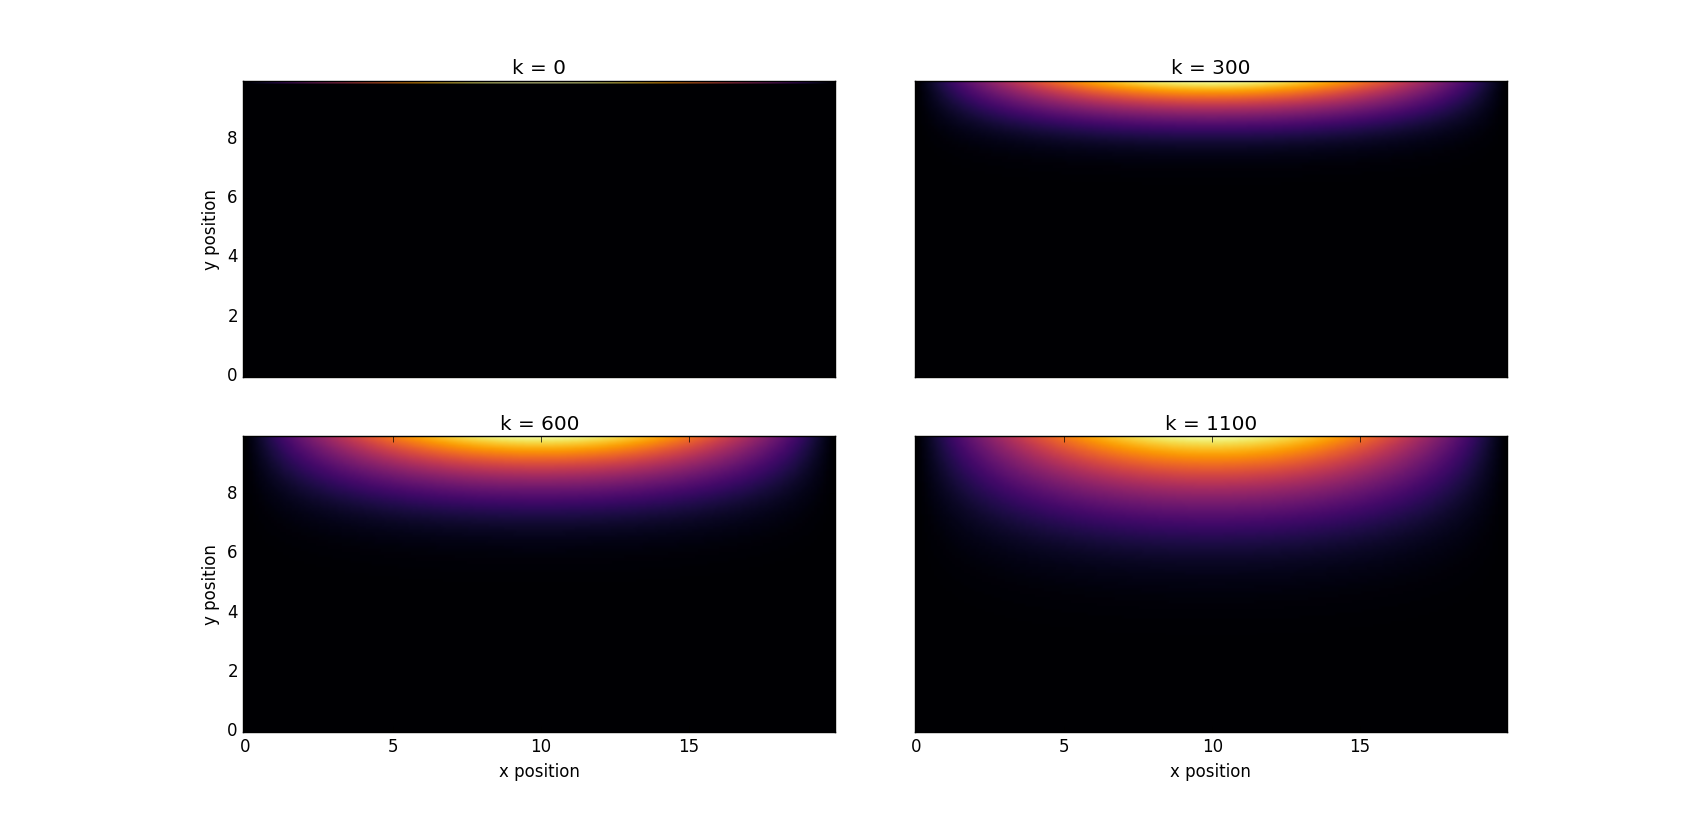
\includegraphics[width=\linewidth]{Relaxation}
\caption{Example of relaxation solving Laplace's equation for the boundaries in Equation 1.2 for a grid of $200 \times 100$ points (domain $[0,20]\times [0,10]$ with steps of 0.1). The k-value represents the number of iterations.}
\end{figure}

\begin{multicols}{2}

\subsection{Relaxation method}

The overall idea of relaxation method is to let an initial guess on a lattice relax and reach an equilibrium corresponding to the the solution (see Figure 1). There are different ways of doing this, and among all of them the following algorithm was defined:

\begin{itemize}
\item Set a grid of points with size $N \times M$
\item Apply the boundary conditions
\item Until the following condition is reached within \footnote{In what follows the parameter $\epsilon$ will be designated as the accuracy. The terms low and high will refer to the value of $\epsilon$. For instance $10^{-4}$ will be a lower accuracy than $10^{-1}$.} $\forall i,j,\ \ | V_{i+1,j} - V_{ij} |>\epsilon \land | V_{i,j+1} - V_{ij}| > \epsilon$ 
\begin{itemize}
\item Copy the first line of the matrix into a vector $\bf x$\rm
\item Go through the grid
\item Copy the first element of the line in $x_0$
\item For each point $(i,j)$ within calculate the new value $V_{ij}$ using Equation 1.6 where 
$V_{i-1,j} = x_{i-1}$ and $V_{i,j-1} = x_{i}$
\item Copy the old value $V_{ij}$ in $x_i$
\item Update $V_{ij}$ with its new value
\end{itemize}
\end{itemize}

\subsection{Analytic solution}

A general way of solving Laplace's equation consists in assuming that we can apply a separation of variables, which means we can rewrite our potential as the following ansatz

\begin{equation}
V(x,y) = X(x) Y(y)
\end{equation}
 
Where the general solutions of X and Y are given by

\begin{equation}
\begin{split}
&X(x) = A \sin kx + B \cos kx\\
&Y(y) = C \sinh ky + D \sinh -ky
\end{split}
\end{equation}

One can show that by applying the 3 trivial boundary conditions the potential can be rewritten under the general form \cite{ComputationalPhysics}

\begin{equation}
V(x,y) = \sum\limits_{n=1}^{\infty} C_n \sin \frac{n\pi x}{x_N} \sinh \frac{n\pi y}{x_N}
\end{equation}

Finally by applying the last boundary condition we see that only the $n=1$ term must be non zero in order to fulfill the equality. We therefore gets the final solution

\begin{equation}
V(x,y) = \frac{1}{\sinh \frac{\pi y_N}{x_N}} \sin \frac{ \pi x}{x_N} \sinh \frac{\pi y}{x_N}
\end{equation}

\subsection{Numerical solution and convergence}

As shown in Figure 2, if the accuracy is low enough the numerical solution converges to the analytic one with good precision. The idea is therefore to determine what low enough means. Obviously since the solution will propagate through the grid and since a high accuracy  implies few iterations we can see that the higher the accuracy the further the solution will be from the analytic one. This is clearly visible in Figure 3 where the numerical solution was computed for different accuracies. As one can see the analytical solution is reached for an accuracy of about $10^{-4}$, but for lower values the solution is really far from what we would expect.\\
This is clearly an issue due to the checking routine. The algorithm checks whether the change between the previous value and the new one is less than the accuracy and if it is the case it stores this information inside another matrix. The algorithm is stopped when all the values verify this condition, but it is obvious that this will always be true for points where the value has not changed (i.e where the solution has no propagated yet). Clearly if the boundary conditions are high enough this should not be a problem since the change between points will be much greater than the accuracy but for boundary conditions with quite low values (such as in this case) this can quickly become a problem.

\end{multicols}
\begin{figure}[H]
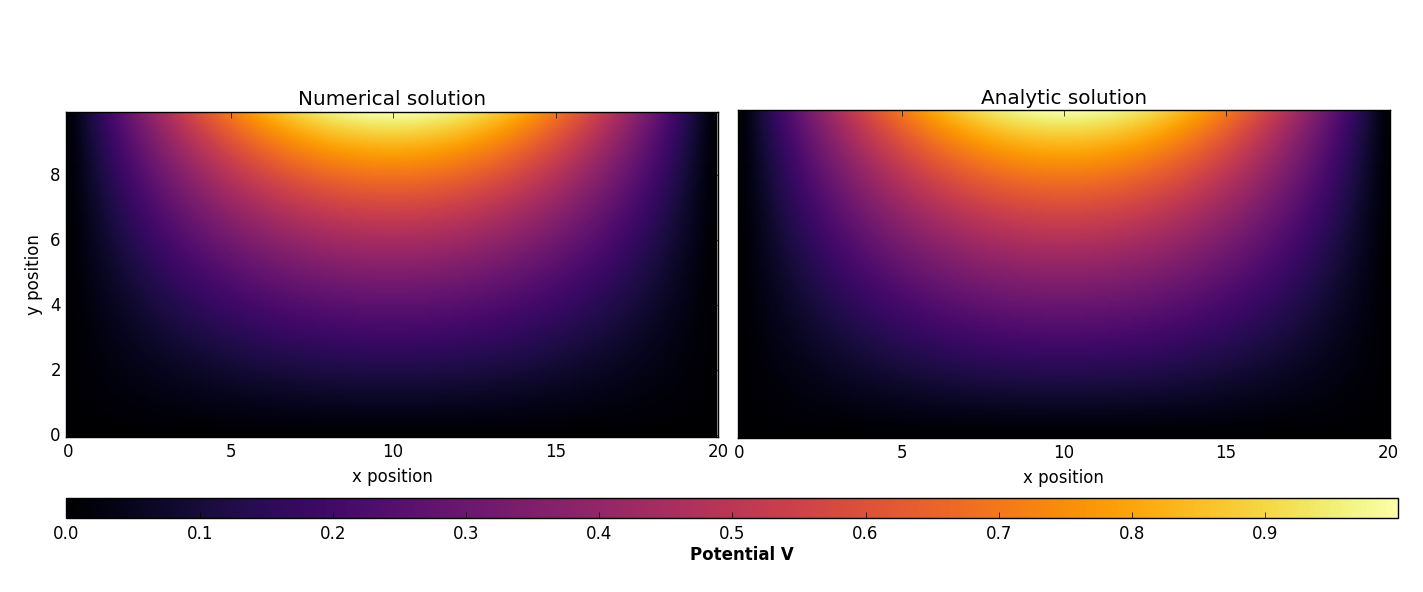
\includegraphics[width = \linewidth]{Laplace_equation}
\caption{Comparison between numerical and analytical solutions to Laplace's equation for the boundaries in Equation 1.2. The step between each point is 0.1 and the numerical solution was determined with an accuracy of $10^{-4}$.}

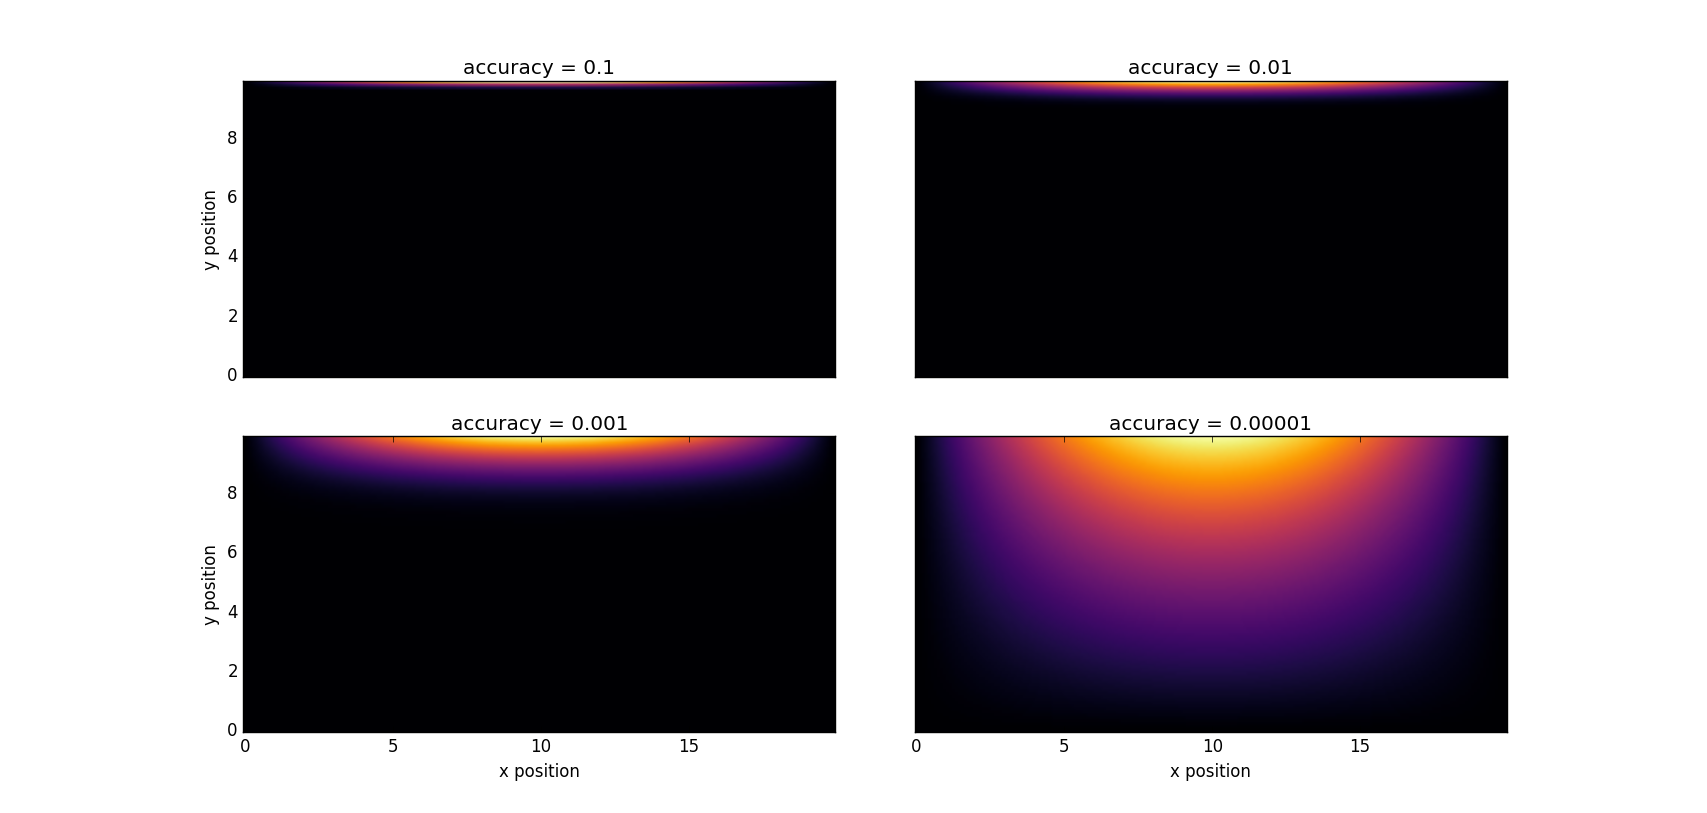
\includegraphics[width = \linewidth]{accuracy_relaxation}
\caption{Numerical solution for four different accuracies. A too low accuracy forbids the solution to propagates far enough which gives a wrong result.}
\end{figure}

\begin{multicols}{2}

\section{Electric Potential and Field inside and around a capacitor}

\subsection{Analytic solution for an infinite sheet capacitor}

We consider a plate capacitor composed of two conducting sheets with dimensions $a \times \infty$ separated by a distance $d$. One of the sheets has a surface charge $+\sigma$ and the other $-\sigma$. 

\begin{figure}[H]
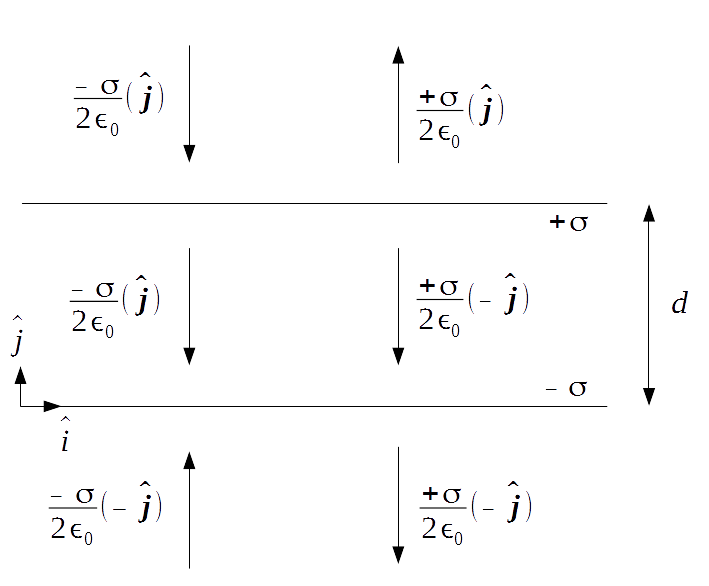
\includegraphics[width=\linewidth]{capacitor}
\caption{The electric fields created by two infinite conducting sheet. One can see that the overall field outside the capacitor is 0 and inside is $\sigma /\epsilon_0$.}
\end{figure}

 It can be shown that the electric field above an infinite conducing sheet of surface charge $\sigma$ lying in the x-y plane is constant and is given by \cite{Cap}

\begin{equation}
\bf E \rm = \frac{\sigma}{2 \epsilon_0} \bf \hat n
\end{equation}
Where $\bf \hat n$ is the normal vector perpendicular to the surface. As shown in Figure 4 if we combine two sheets with opposite surface charge the superposition principle allows us to determine the electric field inside and outside the capacitor

\begin{equation}
\bf E . \hat n \rm = 
\begin{cases}
\frac{\sigma}{\epsilon_0} \ \ & 0 < |y| < d\\
 0 &y \leq 0 ,\ \ y \geq d
\end{cases}
\end{equation}

Moreover we know the electric field is defined as the gradient of the electric potential $\bf E\rm =- \bf \nabla \rm V$ \cite{Electro15}. Therefore by integrating in the three regions and using the fact it is a continuous quantity we get

\begin{equation}
V = 
\begin{cases}
\ \ \ \ V_0 &y \leq 0\\
V_0 + \frac{\sigma}{\epsilon_0}y  & 0 < y < d\\
V_0 + \frac{\sigma}{\epsilon_0}d &y \geq d
\end{cases}
\end{equation}

\subsection{Discussion about expected potential and electric field}

The solution solved in the previous section only applies to a capacitor made of two infinite sheets. This is a good approximation when the finite dimension becomes much larger than the distance between the sheets ($d \ll a$).\\
However, one of the dimensions of the sheets is finite. This implies that side effects will appear for the points near the edge of the conductors. This should not be the case when the points lie close to the bisector plane \footnote{Bisector plane refers here to the plane perpendicular to the sheets and containing the bisector of the finite extent.} of the two sheets since in this case the system has approximately the same symmetries than the infinite model.\\
For a semi-infinite plane capacitor the electric field is quite hard to solve. However from simple electromagnetic laws we can deduce some of its properties. If we look at the symmetries of the system, we see that the infinite extent implies that the electric field and potential will not depend upon z and $\bf \hat k$. 
Furthermore from Maxwell's equations \cite{Maxou} without B-field we can derive two more relations by calculating the divergence and the rotational of $\bf E$. We can summarize these properties as follows

\begin{equation}
\begin{split}
&\bf E \rm = \bf E_x \rm (x,y) + \bf E_y \rm (x,y)\\
&\partial_x E_x = - \partial_y E_y\\
&\partial_y E_x = \partial_x E_y
\end{split}
\end{equation}
Where $E_x = | \bf E_x \rm |$ and $E_y = | \bf E_y \rm |$.

\subsection{Numerical analysis and boundary conditions}

The electric field in free space obeys Gauss' law \cite{GOGO}

\begin{equation}
\bf \nabla . E \rm = \frac{\rho}{\epsilon_0}
\end{equation}
Where $\rho$ corresponds to the volume charge enclosed within an infinitesimal volume. For a capacitor composed of two conducting sheets the volume charge will vanish since all the charges will lie on the sheet. Therefore if we use the definition of the electric potential we get an equation which describes the behaviour of the potential 

\begin{equation}
\nabla^2 V = 0
\end{equation}

This is Laplace's equation and we can therefore solve it numerically using the algorithm defined in the first section. However we need to be careful since this equation only has a sense if we define a domain with the proper boundary conditions. In particular if we were only interested in the potential within and not around the capacitor, we could define our domain as the 2D space spanned by the two conductors. In this case the boundary conditions would match the value of the potential on the interface \footnote{Interface refers to the surface of the conductor. The values on the interface are called interface conditions and are generally different from the boundary conditions.} and could either be 0 or varying linearly on the sides.\\
However since we also want to know the values of the potential outside we need to consider a domain entirely enclosing the capacitor. We can therefore use the values of the potential above and under the conducting sheets to define our boundary conditions. However these boundary conditions do not tell us anything about the values the potential should take on the left and right sides of the domain. For simplicity we define it to be equal to 0 there. This will obviously affect the result, especially near these sides and so it should be taken into account in the analysis of the numerical solution.\\
Finally it needs to be noted that instead of deriving the potential on the interface using a specific surface charge we will for simplicity once again directly apply a certain value of V to the two interfaces. In this case the negatively charged sheet will have a potential of -100V and the positively charged will have a potential of +100V which corresponds to values encountered in real life.

\end{multicols}

\begin{figure}[H]
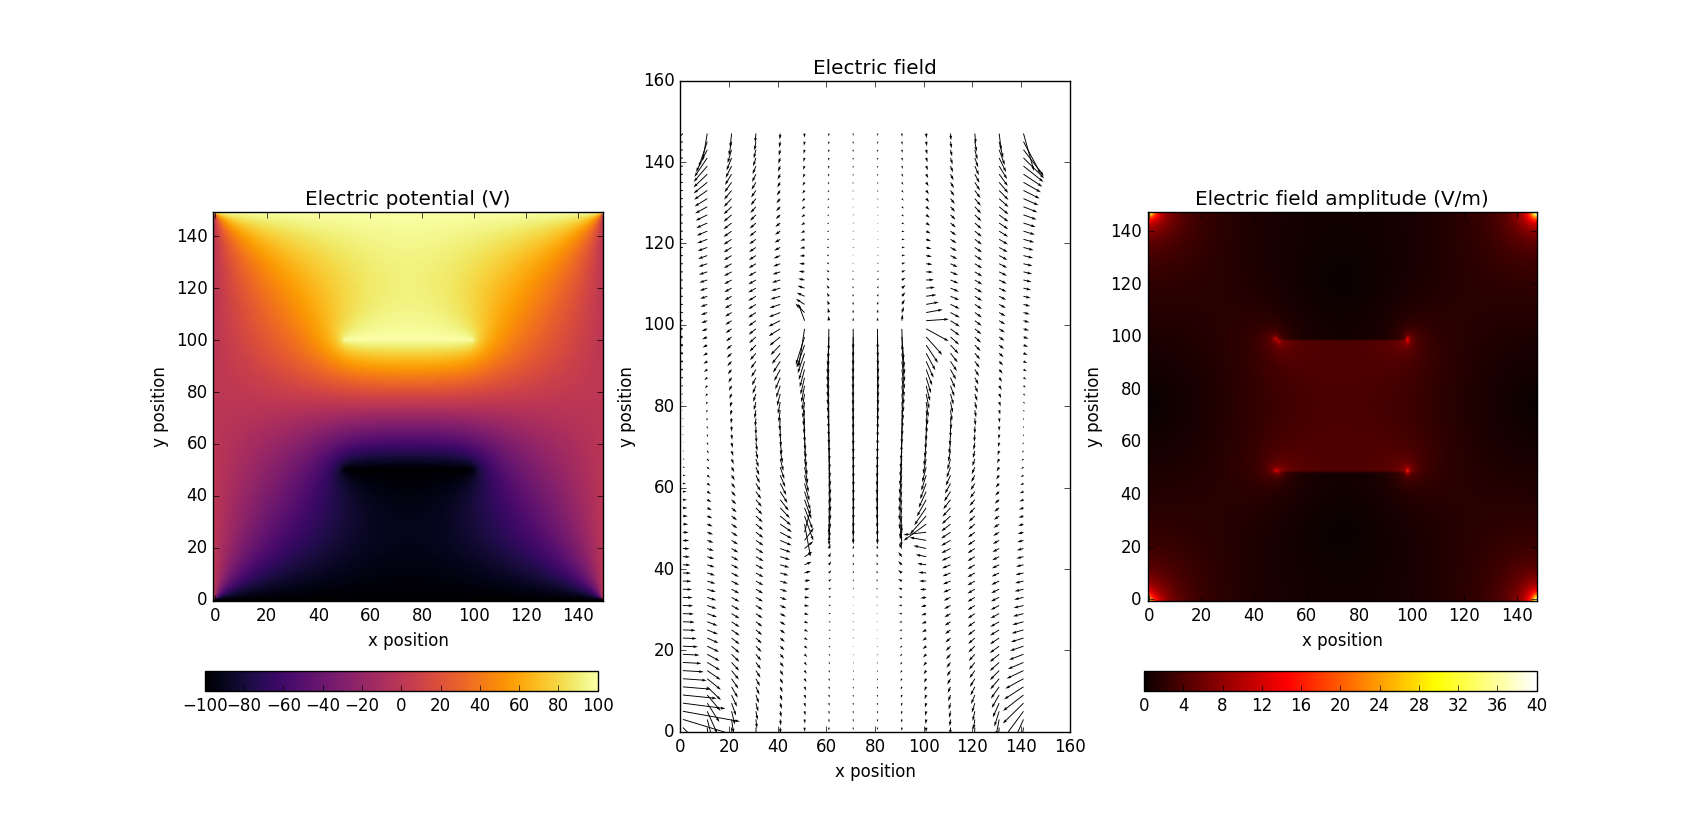
\includegraphics[width=\linewidth]{Electric_field_potential}
\caption{Electric field and potential for a $50 \times 50$ grid within the capacitor with an accuracy of $10^{-3}$. The field is quite constant inside the capacitor and vanishes outside. Side effect are clearly visible in both field and amplitude plots.}
\end{figure}

\begin{multicols}{2}

\subsection{Study of numerical solution}
As seen in the left plot of Figure 5 the potential seems to vary linearly inside from the negatively charged interface to the positive one. Above and under the sheets it is constant and corresponds to the potential of the closest sheet. As we approach the left and right boundaries it reaches 0 which is consistent with the boundary conditions. This could have been avoided by taking other boundary conditions and this is why we will not focus on the regions near the left and right parts of the domain. It is also consistent with the right plot where we can see that the electric field is almost constant within the conductor and reduces to 0  outside.\\
Inside the capacitor the electric field points along the $\bf \hat j$ direction and is slowly bent over when approaching the sides. As one can see in the central plot, side effects are clearly visible especially when approaching the edges of the sheets. The electric field lines are going from the positive end to the negative one which is also consistent with what we would expect.\\
If we look at the case where the two sheets can be approximated as infinite in both directions (see Figure 6), we see that the numerical solution approaches the analytic one derived in Equations 2.2 and 2.3. In particular we see that the potential above and under the sheets corresponds perfectly with what we get in Figure 6b. The electric field is constant within the capactior and vanishes outside. The electri field is pointing in the $\bf \hat j$ direction as expected and side effects are negligible.


\end{multicols}

\begin{figure}[H]
\centering
\subfloat[Similar plot as Figure 5 for a $200 \times 20$ grid within ($d \ll a$). The electric field is constant within the capacitor as expected.]{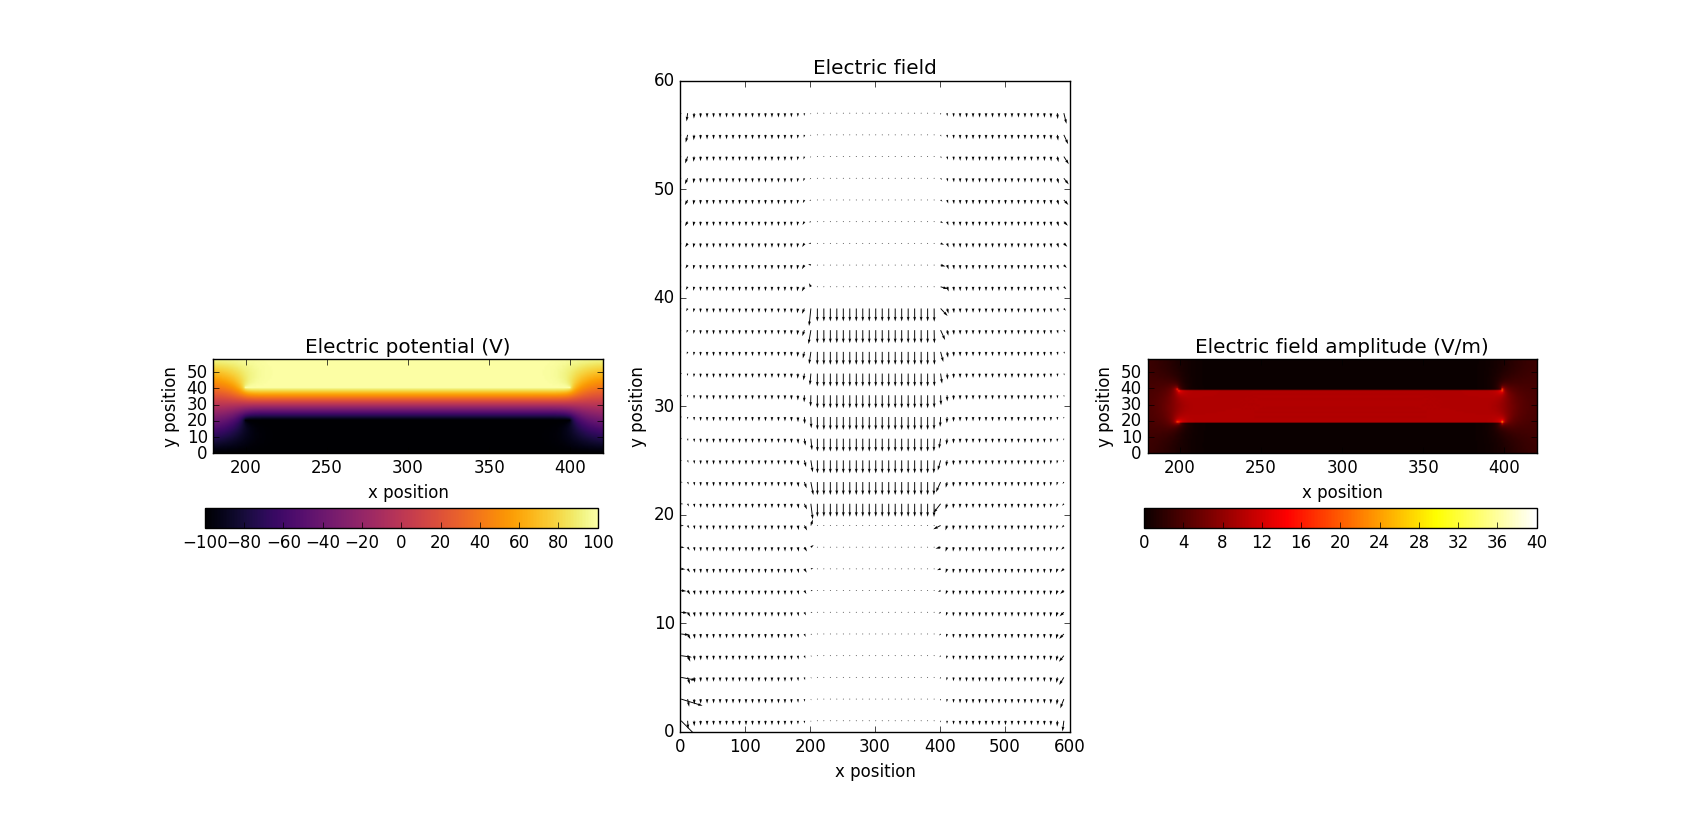
\includegraphics[width=\linewidth]{EFP_200x20}}
\newline
\subfloat[Electric field and potential using the analytic solution when $d \ll a$.]{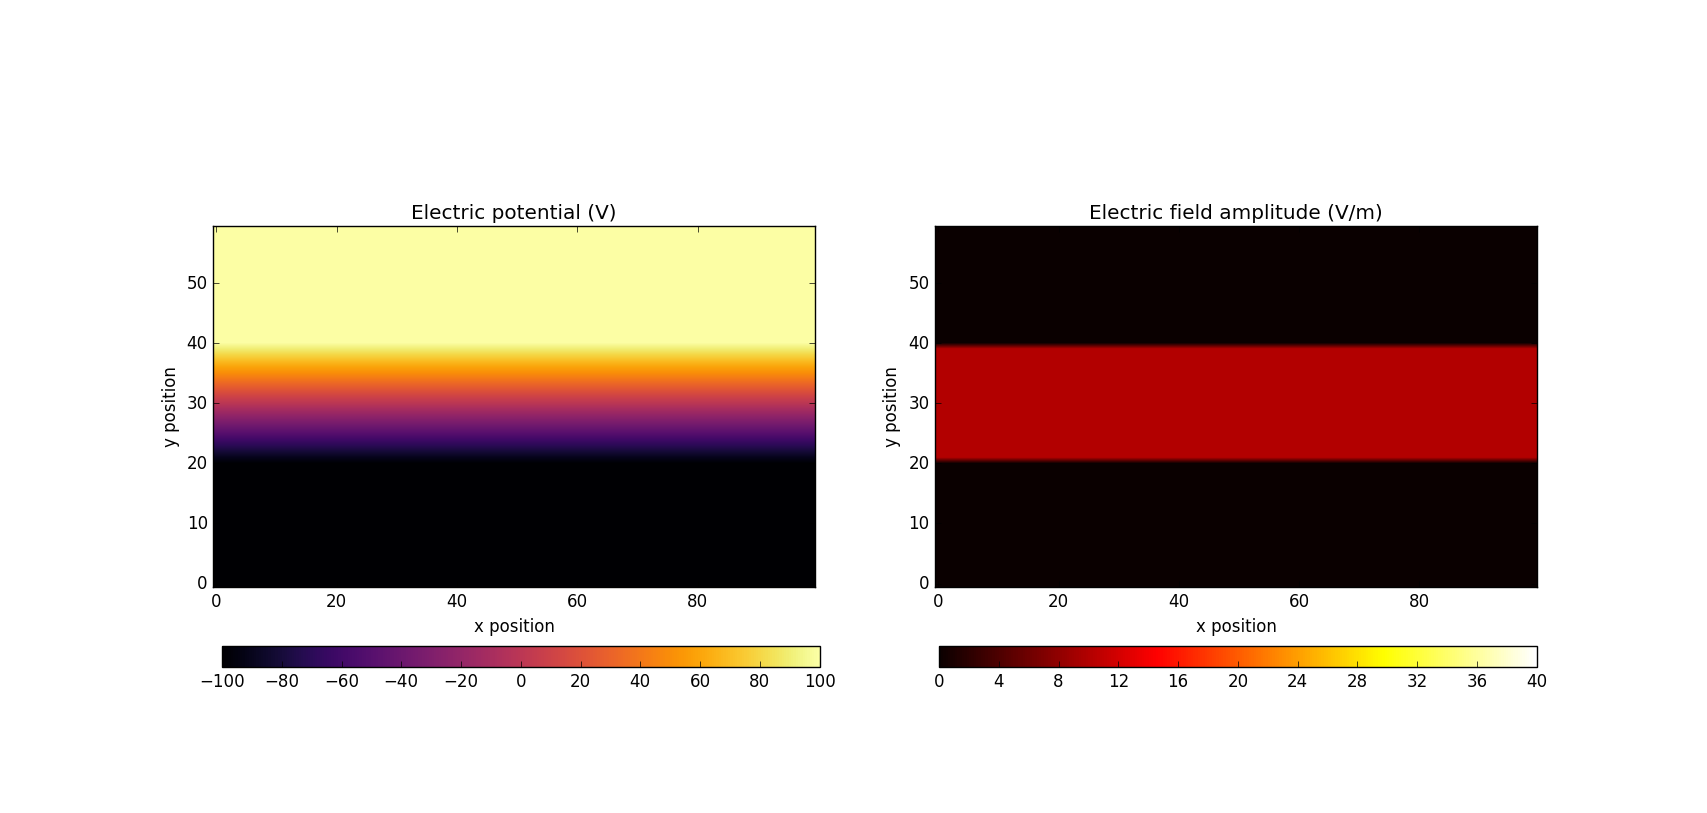
\includegraphics[width=\linewidth]{analytic}}
\caption{Numerical and analytic solutions when the system approaches two infinite sheets in both dimensions.}
\end{figure}

\begin{multicols}{2}

\section{Diffusion problem}
\subsection{Heat equation}

We consider an iron poker of length 50cm with an initial temperature of 20\degree C where one of its ends is put into a furnace with a temperature of 1000\degree C in one case and where the other end is immersed in a block of ice at 0\degree C in the other case (the first end stays in the furnace). The problem is to study how the temperature will evolve along the poker as a function of both time and space. For simplicity we will approximate the poker as a straight line which reduces the 3D problem to a 1D one. We will also make the assumption that there is no heat exchange between the poker and its environment.\\
From the problem we already know both boundary and initial conditions

\begin{equation}
\begin{cases}
\forall x,\ \ T(x,0) = 20 ^\circ \textnormal{C}\\
\forall t, \ \ T(0,t) = 1000 ^\circ \textnormal{C}\\
\forall t, \ \ T(0.5,t) = 20 ^\circ \textnormal{C}
\end{cases}
\end{equation}

Temperature being closely related to heat, studying the problem of the evolution of the temperature along the poker as time evolves is the same as studying the propagation of heat. Therefore we can start from the heat equation \cite{HeatEq}

\begin{equation}
\frac{dQ}{dt} = K A \frac{dT}{dx}
\end{equation}
Where  A is the surface of the poker and K is the thermal conductivity. Since we are only interested in the temperature and not in the heat we need to find a relation between these two quantities. This can be obtained by looking at the heat capacity at constant pressure\cite{HeatEq}

\begin{equation}
C_P = \left ( \frac{dQ}{dT} \right )_P
\end{equation}

This relation is true for any isobaric process which means the pressure must be constant. It might not be obvious why this is the case here and therefore one might argue that it would be more appropriate to consider the heat capacity at constant volume. However we do not need to worry about this since for solids $C_P \approx C_V$.\\
We can rewrite the heat capacity as $m c_P$ where this time $c_P$ is the heat capacity per unit mass. Therefore if we assume that the mass is equally distributed along the poker we can rewrite our heat capacity for an infinitesimal bit of length $dx$ as

\begin{equation}
C_P = \rho A  c_P dx
\end{equation}
Where $\rho$ is the density of the iron in our case. Finally putting everything together leads to the equation describing the temperature along the road and over time

\begin{equation}
\partial_t T= \alpha \partial_x^2 T
\end{equation}
With $\alpha = \frac{K}{\rho c_P}$ the thermal diffusivity.

\subsection{Ansatz for the analytical solution}
We know from the heat equation that if the time derivative vanishes we have a temperature distribution $T = Ax + B$ with A and B two constants. In particular we expect our system to reach an equilibrium where the temperature will stay stable and therefore we can infer this solution will be reached for $t \rightarrow \infty$. We also know that the temperature will spread along the poker and that the temperature gradient will be high for low t near the end inside the furnace. Hence we can infer that it will behave as a decreasing exponential at the beginning until the linear part takes over. Thus, we assume that the spatial part can be written as the following ansatz

\begin{equation}
T = C e^{-\lambda x} + Ax + B
\end{equation}
Whith A, B and C three constants.

\subsection{Numerical analysis and stability}

We want to solve the heat equation numerically. Therefore we need to discretize the equation which can be done via two different schemes\cite{NumHeat}

\begin{equation}
\begin{split}
&\frac{T_i^{n+1} - T_i^n}{\Delta t} \approx \alpha \frac{T_{i+1}^n - 2 - 2T_i^n + T_{i-1}^n}{(\Delta x)^2}\\
&\frac{T_i^{n+1} - T_i^n}{\Delta t} \approx \alpha \frac{T_{i+1}^{n+1} - 2T_i^{n+1} + T_{i-1}^{n+1}}{(\Delta x)^2}
\end{split}
\end{equation}
Where the index refers to space and the exponent to time ($T(x,t) \leftrightarrow T_i^n$).
These two equations are obtained by using the Taylor expansions in Equation 1.4. The first equation is named fully explicit and the second one fully implicit. The only difference between them is that the second one is evaluated at $t = n+1$ when the first one is evaluated at $t=n$.\\
We will use the second equation to solve numerically the equation, the reason being that the second equation is unconditionally stable (i.e. the stability does not depend upon the choice of the time step). Stability can be studied by looking at von Neumann Stability Analysis\cite{NumStab}. We consider that each coefficient in the difference equation is constant and therefore each solution can be written under the following form

\begin{equation}
 T_i^n = \zeta ^n e^{ikj \Delta x}
\end{equation}
Where k is a spatial wave number and $\zeta$ a complex number. The equation will be unstable for $| \zeta | > 1$ and therefore by substituting this expression into the equation we can find a stability criterion. In particular it can be shown that the stability criterion for the two equations in Equation 3.7 are respectively given by\cite{NumHeat}

\begin{equation}
\begin{gathered}
\zeta = 1 - \frac{4\alpha \Delta t}{(\Delta x)^2} \sin ^2 \frac{k \Delta x}{2}\\
\zeta = \left ( 1 + 4 \frac{\alpha \Delta t}{(\Delta x)^2} \sin ^2 \frac{k \Delta x}{2} \right )^{-1}
\end{gathered}
\end{equation}

Where the requirement $| \zeta | \leq 1$ leads to the stability criterion $\Delta t \leq \frac{(\Delta x)^2}{2\alpha}$ for the first equation and $\Delta t \in \mathbb{R} $ for the second one.\\
Hence we can see that the second equation is actually stable for any value of $\Delta t$ when for the first one it will depend on $\Delta x$. Now that we know which equation to use, we can rearrange it in a more convenient form

\begin{equation}
\left ( 1 + \frac{2 \alpha \Delta t}{(\Delta x)^2} \right ) T_i^{n+1} - \frac{\alpha \Delta t}{(\Delta x)^2} ( T_{i-1}^{n+1} + T_{i+1}^{n+1} ) = T_i^n
\end{equation}

If we define a vector $\bf T^n$ of size I containing all the values $T_i^n$ we see we can actually rewrite this as a matrix equation

\begin{equation}
\begin{gathered}
A \bf T^{n+1} \rm = \bf T^n\\
\rm \begin{pmatrix}
1 & 0 & \cdots & \cdots & 0\\
\bf v & 0 & \ddots & & \vdots \\
0 & \bf v & \ddots & \ddots & \vdots\\
\vdots & & \bf v & 0 & 0\\
0 & \cdots & \cdots & 0 & 1
\end{pmatrix}
\begin{pmatrix}
T_1^{n+1}\\
\vdots\\
\vdots\\
\vdots\\
T_I^{n+1}
\end{pmatrix}
=
\begin{pmatrix}
T_1^{n}\\
\vdots\\
\vdots\\
\vdots\\
T_I^{n}
\end{pmatrix}
\end{gathered}
\end{equation}
Where $\bf v \rm = \left ( \frac{-\alpha \Delta t}{(\Delta x)^2} \ \ 1 + \frac{2\alpha \Delta t}{(\Delta x)^2} \ \ \frac{-\alpha \Delta t}{(\Delta x)^2} \right )$.

Therefore we can solve this equation by discretizing the poker in a set of points, applying boundary and initial conditions from Equation 3.1 and using the LU method algorithm from the GSL library\cite{GSL}. Each $\bf T^{n+1}$ will correspond to the solution of the heat equation at time $t = n+1$.
\end{multicols}

\begin{figure}[H]
\centering
\subfloat[Case with $T(0.5,t) = 20^\circ C$.]{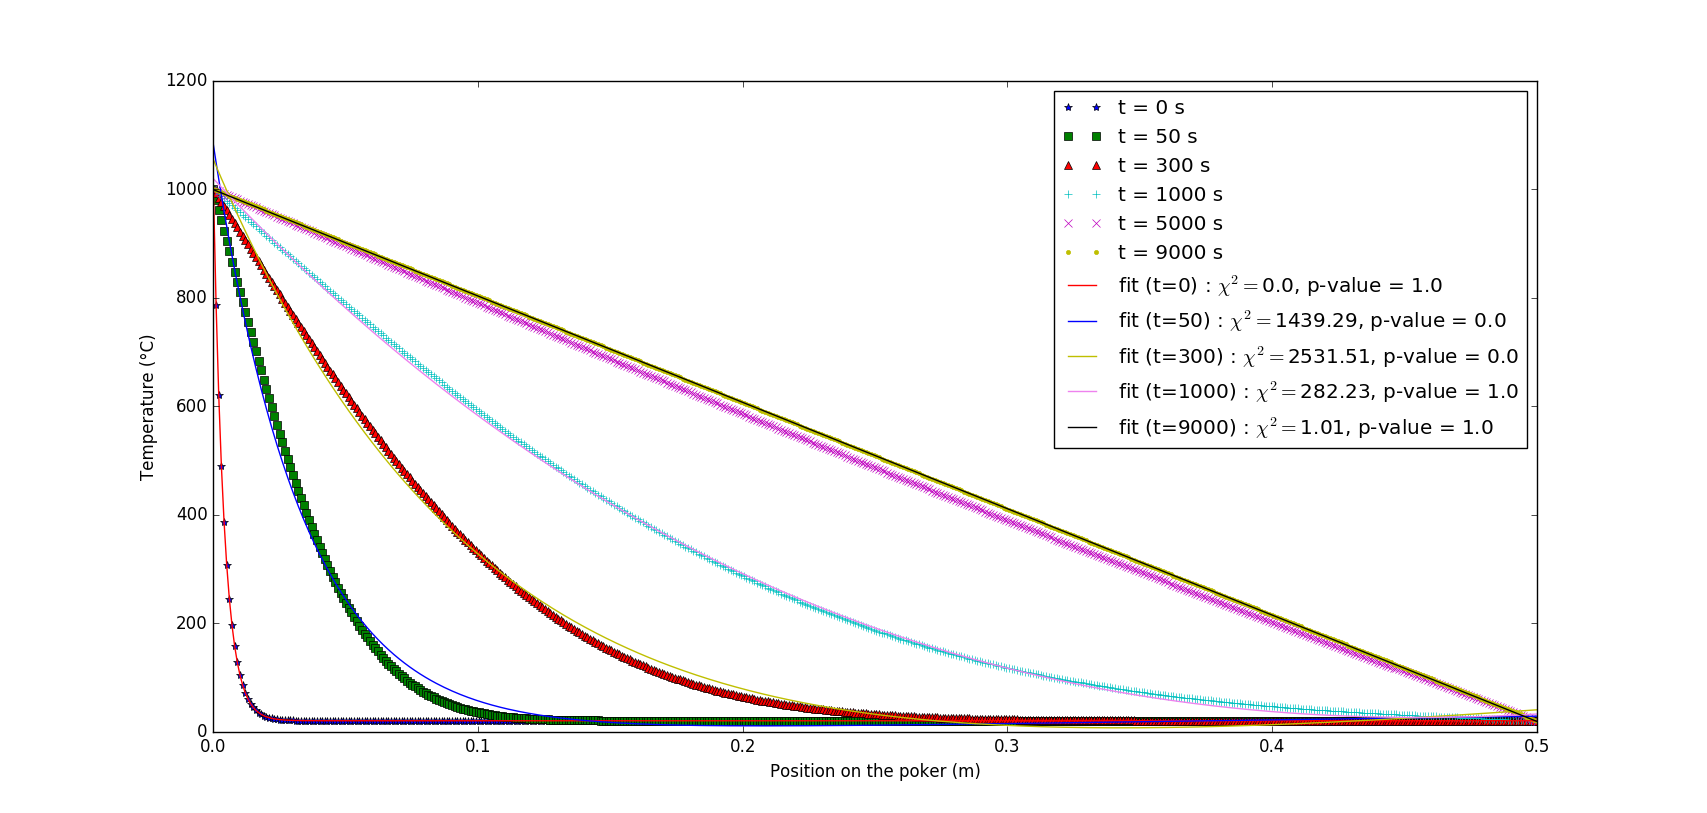
\includegraphics[width=\linewidth]{Temperature}}
\newline
\hspace{1pt}
\subfloat[Case with $T(0.5,t) = 0^\circ C$.]{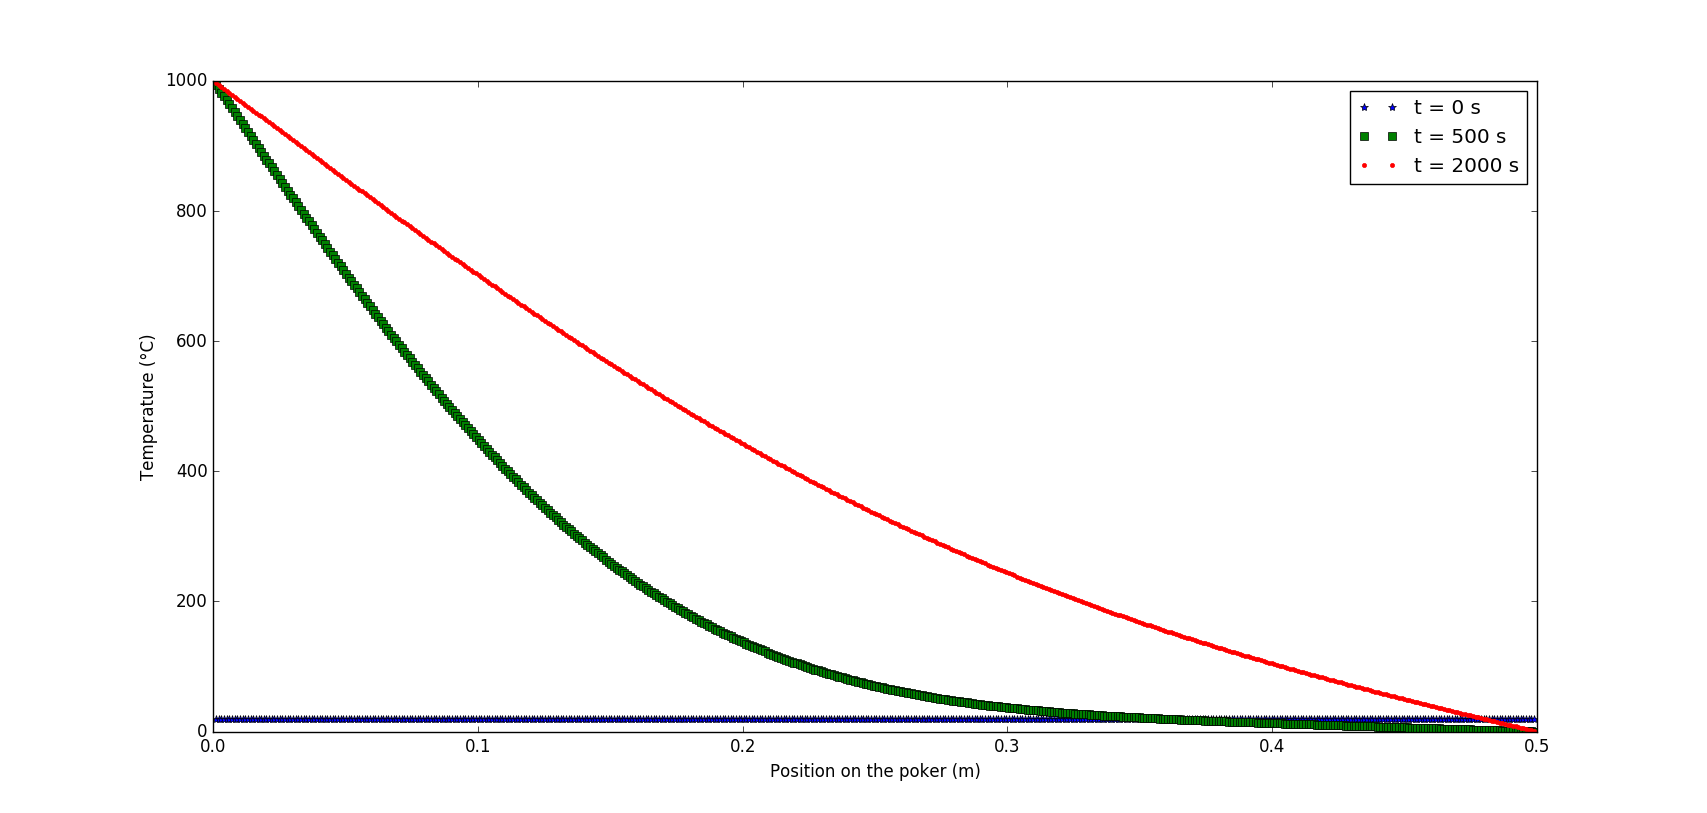
\includegraphics[width=\linewidth]{Temperature0}}
\caption{Distribution of the temperature along the poker for the two cases and for different time. The fits corresponds to Equation 3.6. The solution behaves like a decreasing exponential at the beginning and converges to a decreasing linear function.}
\end{figure}

\begin{multicols}{2}

\subsection{Study of the numerical solution}

The two problems were solved with a set of 500 points using Equation 3.11. As one can see in Figure 7a, the temperature distribution behaves as an exponential for low t. As time increases the distribution slowly reaches an equilibrium which corresponds to a linear distribution along the poker.\\
Equation 3.6 fits perfectly for low and high t but seems to be less accurate for intermediate time. This is probably due to the fact that Equation 3.7 that we used to derive the numerical solution is actually an approximated equation. Since the temperature gradient is really high for low t and almost 0 for high t, the discretized equation should be quite accurate. However for intermediate time the temperature spreads through the poker and therefore the change in temperature is more likely to be affected by the error induced by the discretization.\\
We can see in Figure 7b that the solution does also converge towards a linear solution as expected. However in this case there are two temperature gradients: one from the hot end and one from the cold end. As expected the hot end gradient will be much larger than the other one due to the temperature difference near those points. It still does impact the way the temperature is distributed. In particular we can see that Equation 3.6 will not properly describe the distribution in this case since there will be another exponential at the cold end.

\end{multicols}


\newpage
\begin{thebibliography}{1}
\bibitem{ComputationalTechnics}
P K MacKeown, D J Newman, 1988, Computational Technics in Physics, Adam Hilger, 51-52
\bibitem{ComputationalPhysics}
Rubin H. Landau, Manuel J. Paez, 1997, Computational Physics Problem solving with computers, Wiley-Interscience, 348-349
\bibitem{Cap}
I.S Grant, W. R Phillips, Electromagnetism, 1990, 41
\bibitem{Electro15}
Leonard Eyges, 1972, The Classical Electromagnetic Field, Dover, 15
\bibitem{Maxou}
I.S Grant, W. R Phillips, Electromagnetism, 1990, 356
\bibitem{GOGO}
I.S Grant, W. R Phillips, Electromagnetism, 1990, 2
\bibitem{HeatEq}
Mark W. Zemansky, Richard H. Dittman, 1997, Heat and Thermodynamics, 90-91
\bibitem{NumHeat}
William H. Press, Brian P. Flannery, Saul A. Teukolsky, William T. Vetterling, 1988, Numerical Recipes The Art of Scientific Computing, 636-637
\bibitem{NumStab}
William H. Press, Brian P. Flannery, Saul A. Teukolsky, William T. Vetterling, 1988, Numerical Recipes The Art of Scientific Computing, 625-626
\bibitem{GSL}
GNU Scientific Library (GSL), LU decomposition, \url{https://www.gnu.org/software/gsl/manual/html_node/LU-Decomposition.html}
\end{thebibliography}
\end{document}
